\chapter{Appendix - SuperGlue API}
\label{appendix}

\section{Posting media to SuperGlue}
Media is posted to SuperGlue using an HTTP POST request to \url{http://super-glue.media.mit/post_video}. It accepts a JSON\cite{json} encoded document in which the only mandatory fields are \textit{mediaurl}, \textit{title} and \textit{source}. Example: 

<TODO: all the JSON is commented out because of a plugin error >

% {
% 	"title" : "Cradles to Crayons",
% 	"media_url": "https://dl.dropboxusercontent.com/u/3829383/c2c.mov",
% 	"source": "this-is-how"
% }

Optionally, we can add subtitles though if not provided they will be created from a transcript. 

The return value is also JSON encoded and should include a result and media id if the result is ``ok''.

% {
% 	"result" : "ok",
% 	"id": "57ba3a303c85800001d5e16a",
% }

For debugging purposes, we can now see the metadata document in \url{http://super-glue-dashboard.herokuapp.com/} 

\begin{figure}[thpb]
  \centering
  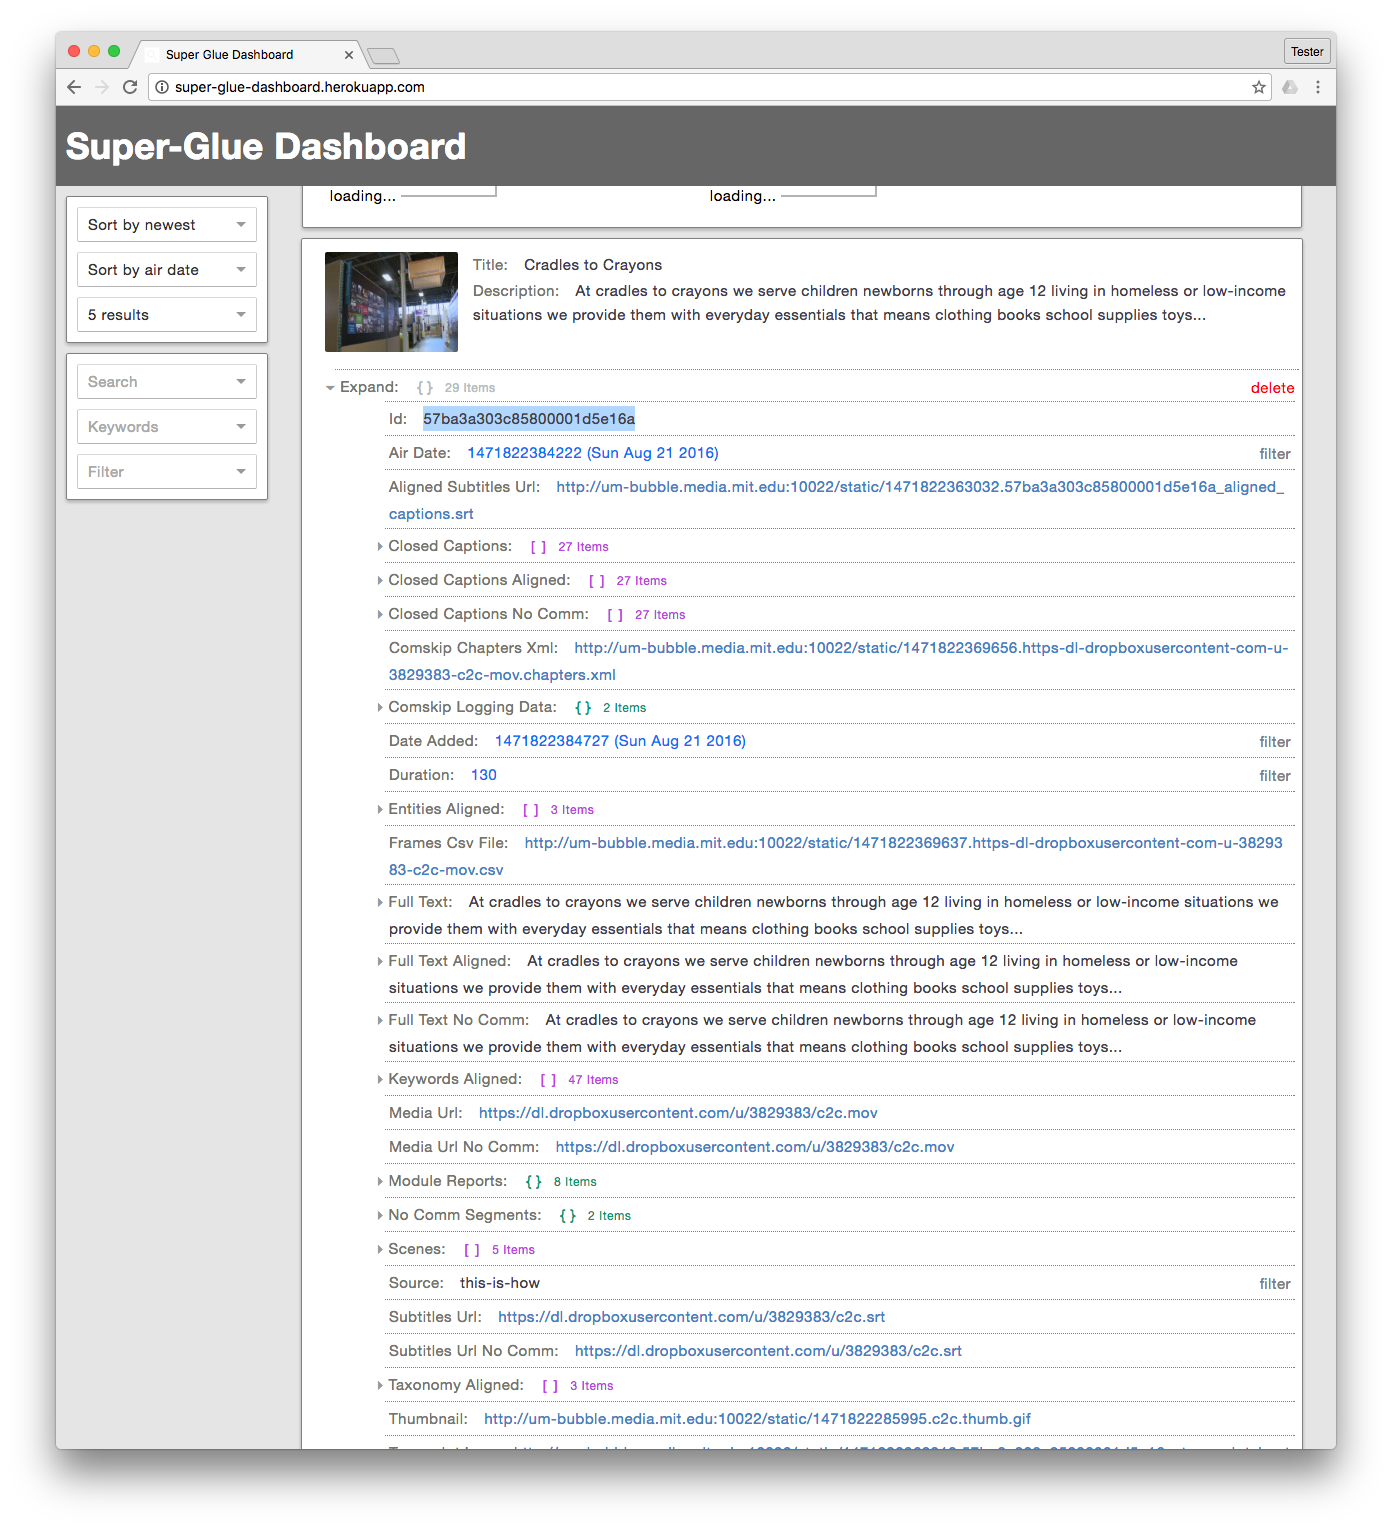
\includegraphics[width=3in]{figures/super-glue-dashboard.png}
  \caption{SuperGlue dashboard displaying metadata}
  \label{fig_superglue_dashboard}
\end{figure}

This document is initialized with the request data and will grow as metadata is generated through completion of modules. 

\section{Querying for metadata from SuperGlue}
